\documentclass[12pt,a4paper]{article}
\usepackage{indentfirst,latexsym,graphicx}
\usepackage[utf8]{inputenc} % Включаем поддержку UTF8
\usepackage[russian]{babel}
\usepackage{amssymb,amsmath}
\graphicspath{{img/}} % тут картинки твои
\usepackage[left=2cm,right=2cm,top=2cm,bottom=2cm,bindingoffset=0cm]{geometry}
\usepackage{amsmath, amssymb, amsthm}

\begin{document}
Принципиальная схема:
\begin{center}
        \begin{figure}[h!]
                \center{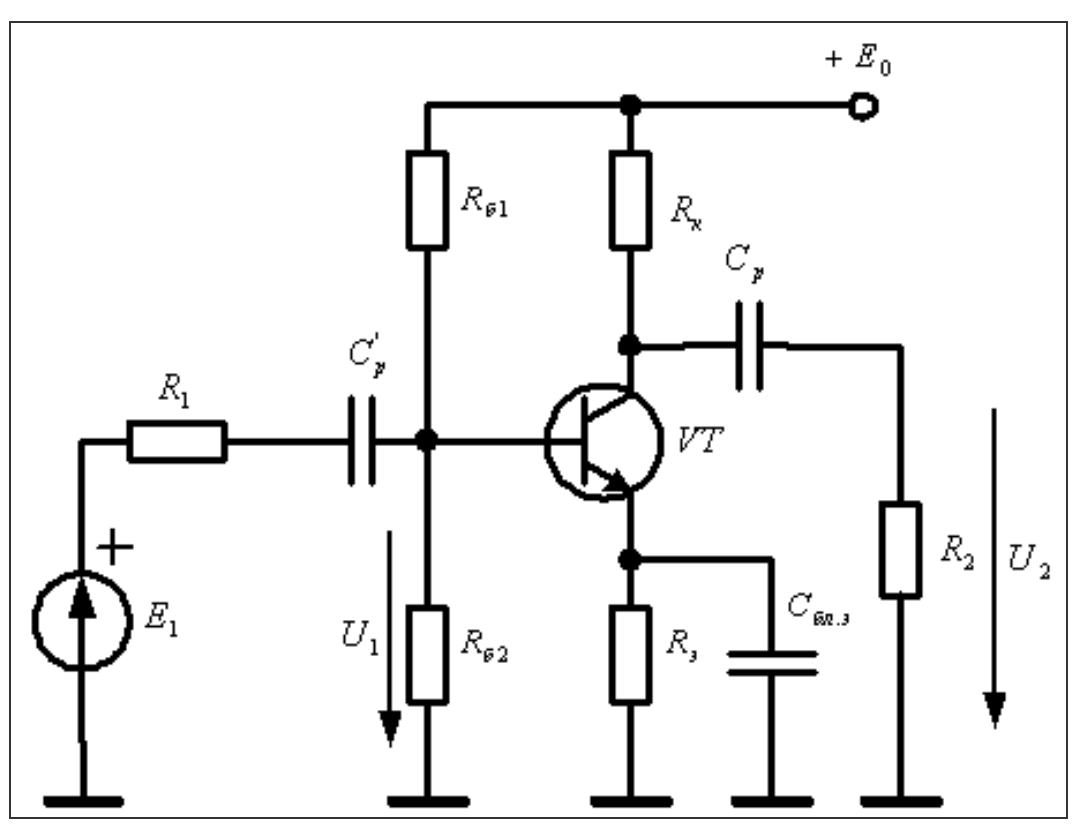
\includegraphics[scale=0.2]{oe.png}}
                \caption{Если ошиблись в назначении сопротивления резистора Rе усилтельного каскада, то к чему это может привести?}
        \end{figure}
\end{center}

//Здесь рассматриваем каскад ОЭ + эквив схема

ВСТАВКА КАРТИНКИ pict19_1.png

$I_k/I_b=B$ - коэффициет усиления по току

Основное назначение резистора Rе -> ОС (по току отриц)
Это также служит для термостабилизации, так как изменение параметров транзистора в диапазоне температур вызывает смещение РТ покоя по нагрузочной прямой, а значит могут возникать нелинейные искажения или даже отсечка выходного сигнала.

При вставке Rэ изменятся некоторые параметры каскада:
$R_\textit{вхтроэ}=r_b+(B+1)(r_e+R_e)$
=> \downarrow Ku и \downarrow Ki - как и должно быть при ООС.
$K_\textit{u_os} = K_u/(1+\beta Ku)$
$K_\textit{u_oe} = B[R_k||R_н]/(r_b+(B+1)(Re+r_e) = [R_k||R_н]/(Re))$

$Re << R_k||R_н$
при Rн = \infty (холостой ход)  $K_\textit{u_oe} = R_k/R_e$ - выражение, характеризующее глубокую ОС, когда усилительные параметры не зависят от свойств цепи прямой передачи и определяется коэффициентом ОС: $\beta = R_e$
Для исключения ОС || - но Rэ ставят Сэ.

Температура растет => $I_\textit{k0}$ в К растет => растет $U_\textit{e0} = I_\textit{э0}R_\textit{e} = I_\textit{k0}R_\textit{e}$
$U_\textit{b0}$  фиксируется в Б сопротивлениями R1 и R2
$U_\textit{be} = (U_\textit{b0}-U_\textit{e0}\uparrow)$ уменьшается => $I_\textit{b0}$ уменьшается => $I_\textit{k0} = [BI_\textit{b0}+(1+B)I_\textit{kb0}]$ уменьшается => ООС c помощью резистора Re препятствует изменению тока К.

$\delta I_\textit{k0} = S[\delta I_\textit{kb0}+\delta U_\textit{be0}/(R_e+R_b)+I_\textit{e0}/(1+B)+\delta B/B$ 

(*) $S = B/(1+B(R_e/(R_e+R_b)))$ - коэффициет нестабиьности, характеризующий эффективность ОС.
При Re->0,  S = Smax =B
Re >> Rb -схема с идеальной термостабализацией S=Smin=1

Таким образом, при re << Re, B >> 1, rb << BRe => Rвх = BRe, Ku = Rk/Re в схеме с ОЭ режим работы каскада изменяется, Ku уменьшается  - отрицательная ОС, но увеличивается входное сопротивление каскада. 
При Re -> 0 коэффициент нестабильности достигает максимума => исключение ООС => возникают линейные искажения, есть вероятность отсечки выходного сигнала.
Для типичных значений Rk||Rн = 3 \div 5 кОм, R0 <= 0.5 кОм.
\end{document}
